\documentclass[12pt]{article}
\usepackage[a4paper, total={6in, 9in}]{geometry}
\usepackage{graphicx}
\graphicspath{ {./images/output/} }
\usepackage{caption}
\usepackage[english]{babel}
\usepackage{titling}
\usepackage{float}
% \usepackage{amsmath}
% \usepackage{minted}
% \usepackage{multicol}
% \usepackage{array}
% \usepackage{setspace}
% \usepackage{placeins}

% \usepackage{lipsum}

\title{Study of Single Phase Bridge Inverter Using Simulink}
\author{}
\date{}

\pagenumbering{gobble}
\begin{document}
\vspace*{\fill}
\begin{center}

    \emph{Heaven's Light is Our Guide} \\
    \textbf{Rajshahi University of Engineering and Technology} \\

    \begin{figure}[H]
        \centering
        
\includegraphics[scale=.34]{images/RUET_logo.png}
        \label{fig:ruet_logo}
    \end{figure}
    \vspace{5mm}

    \textbf{Course Code}\\
    ECE 3206\\
    \vspace{3mm}
    \textbf{Course Title}\\
    Industrial Electronics Sessional

    \vspace{5mm}
    \textbf{Experiment Date:} {January 13, 2025},\\
    \textbf{Submission Date:} {February 10, 2025}\\

    \vspace{5mm}
    \textbf{Lab Report 3: \\
        Study of Thyristor Characteristics R, RL Load}

    \vspace{15mm}

    \begin{tabular}{c|c}
        \textbf{Submitted to} & \textbf{Submitted by} \\
        Md. Faysal Ahamed     & Md. Tajim An Noor     \\
        Lecturer              & Roll: 2010025         \\
        Dept of ECE, Ruet     &                       \\
    \end{tabular}

\end{center}
\vspace*{\fill}


\pagebreak

\tableofcontents

\pagebreak
\pagenumbering{arabic}
\maketitle

\section*{Theory}
\addcontentsline{toc}{section}{Theory}
The Single Phase Bridge Inverter is a power electronic circuit that converts DC input into AC output, enabling the operation of AC loads from a DC source. It is widely used in industrial applications for driving AC motors, renewable energy systems, and uninterruptible power supplies (UPS) \cite{rashid2013power}.

\subsection*{Working Principle}
The circuit consists of four switches (typically IGBTs or MOSFETs) arranged in an H-bridge configuration. By controlling the switching sequence, the polarity of the DC voltage applied to the load is alternated, generating an AC output. The output waveform can be controlled to approximate a sinusoidal waveform using techniques such as Pulse Width Modulation (PWM) \cite{sen1987principles}.

\subsection*{Behavior with R Load}
For a purely resistive load, the current waveform follows the voltage waveform. The output voltage is a controlled AC waveform, and the power delivered to the load is proportional to the RMS value of the output voltage. The switching pattern directly determines the quality of the output waveform \cite{mohan2003power}.

\subsection*{Behavior with RL Load}
For an inductive load, the current lags the voltage due to the inductance. This lag affects the switching transitions, as the current may continue to flow through the freewheeling diodes even after the switches are turned off. The output voltage waveform is still controlled by the switching pattern, but the current waveform exhibits a phase lag \cite{bose2002modern}.

\subsection*{Applications}
\begin{itemize}
    \item Speed control of AC motors
    \item Renewable energy systems (e.g., solar inverters)
    \item Uninterruptible Power Supplies (UPS)
    \item Industrial power regulation
\end{itemize}

The use of MATLAB/Simulink for simulation allows for detailed analysis of the inverter's behavior under different load conditions, enabling optimization for specific applications \cite{mathworks2023simulink}.


\section*{Required Equipments/Software}
\addcontentsline{toc}{section}{Required Equipments/Software}
\begin{itemize}
    \item MATLAB/Simulink
    \item DC Voltage Source
    \item IGBTs
    \item Capacitors
    \item Diodes
    \item Resistive Load (R)
    \item Inductive Load (RL)
    \item Pulse Generator for firing angle control
    \item Measurement Blocks (Voltage and Current)
    \item Scope for waveform visualization
\end{itemize}

\section*{Circuit Diagrams}
\addcontentsline{toc}{section}{Circuit Diagrams}
\begin{figure}[H]
    \centering
    % 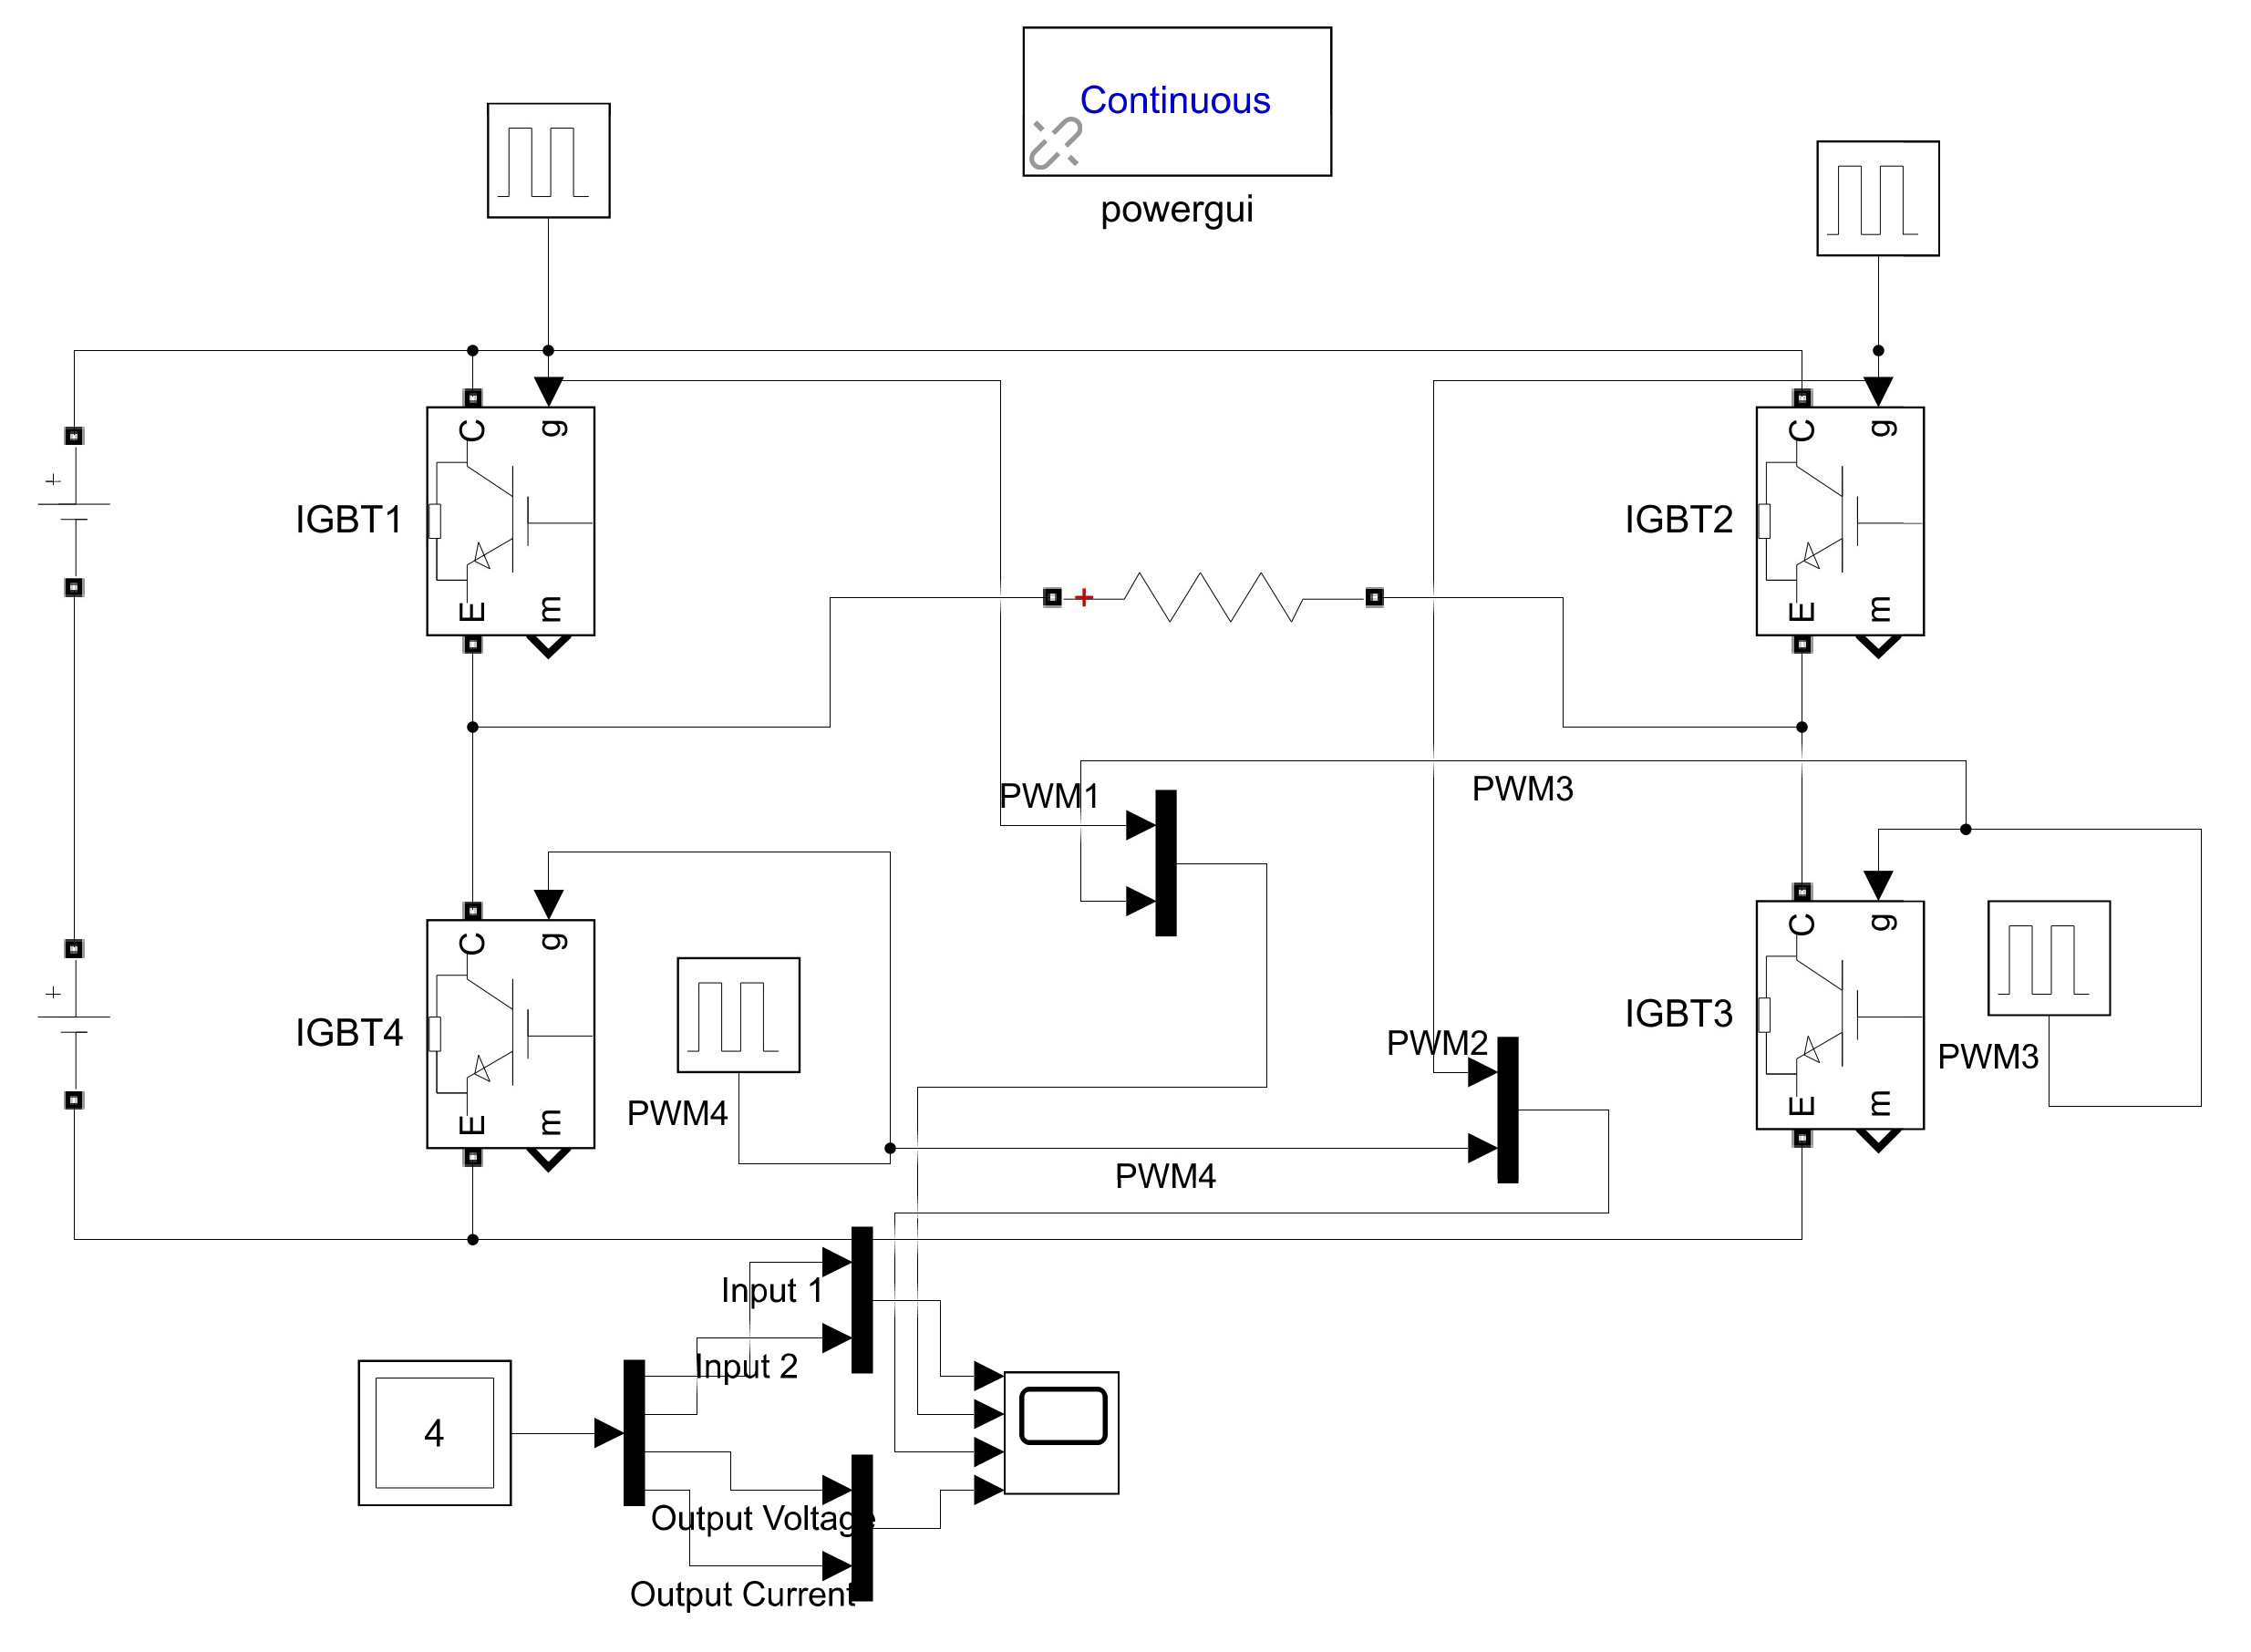
\includegraphics[width=\textwidth]{ckt.png}
    \caption{Single Phase Full Bridge Inverter Circuit}
\end{figure}

\section*{Observations}
\addcontentsline{toc}{section}{Observations}
\begin{itemize}
    \item For the R load, the output voltage waveform is a controlled AC waveform, with the RMS value depending on the switching pattern of the inverter.
    \item Increasing the modulation index for the R load increases the effective RMS voltage and power delivered to the load.
    \item For the RL load, the output voltage waveform is controlled by the switching pattern, but the current waveform lags due to the inductance.
    \item The lagging current in the RL load causes the freewheeling diodes to conduct during the switching transitions.
    \item MATLAB/Simulink simulations show the impact of switching patterns on the output voltage and current waveforms for both R and RL loads.
    \item The circuit demonstrates effective conversion of DC to AC power, enabling operation of AC loads from a DC source.
    \item The behavior of the circuit under different load conditions highlights the importance of considering load characteristics in inverter design and operation.
\end{itemize}


\subsubsection*{Outputs}
\begin{figure}[H]
    \centering
    % 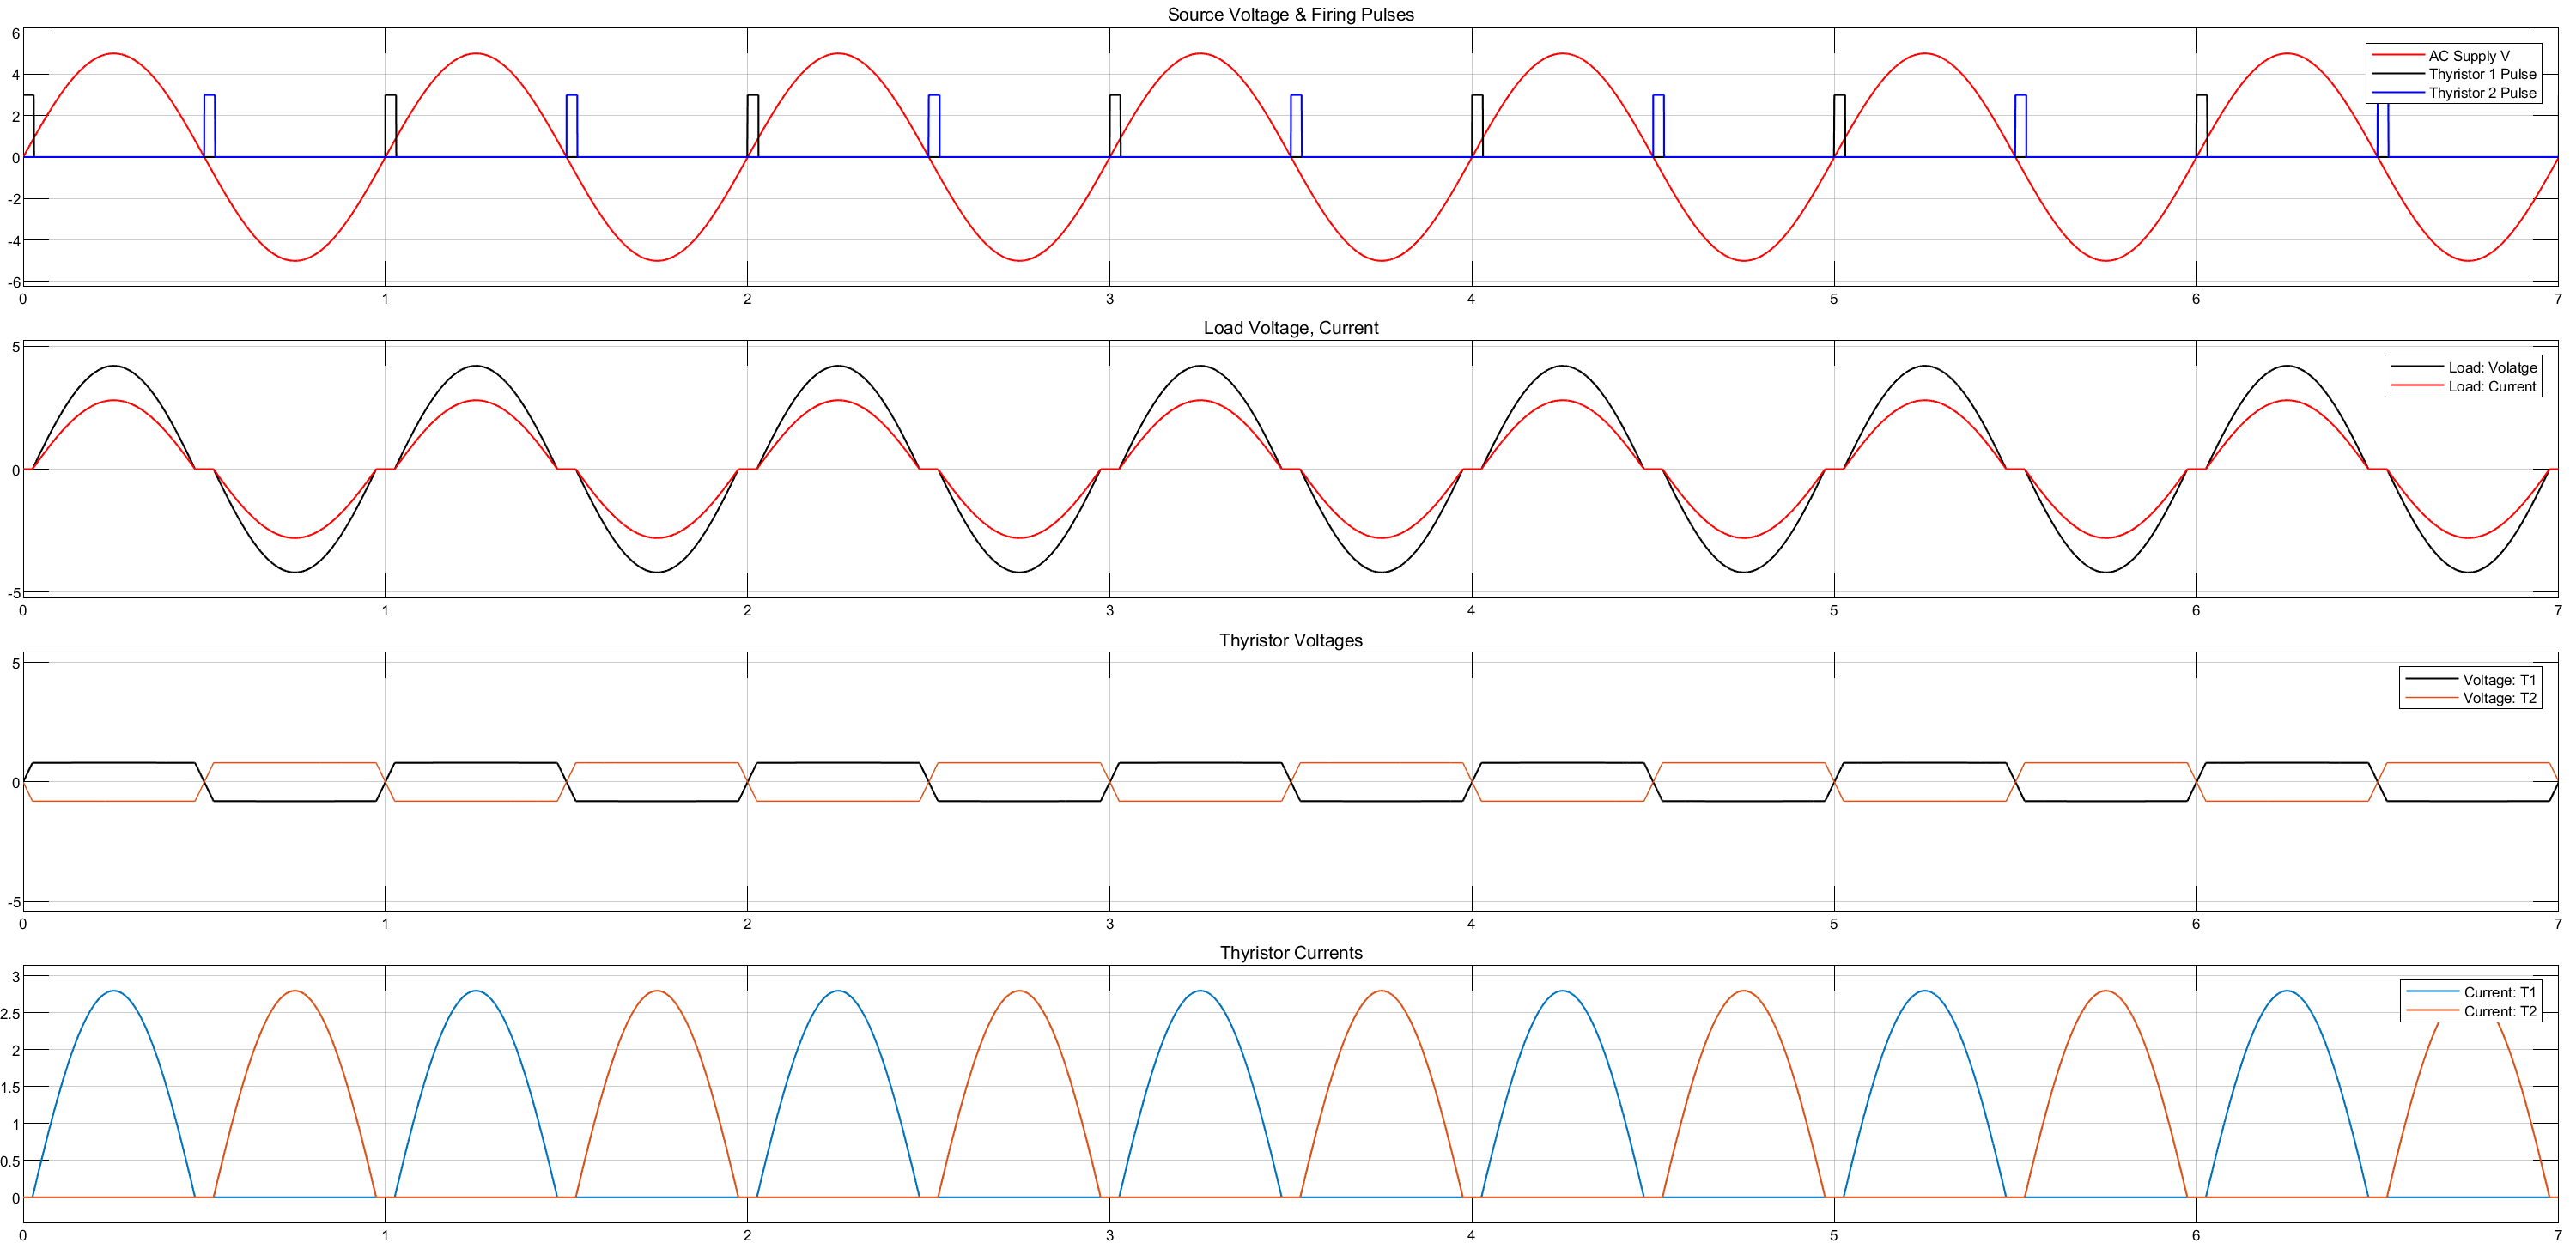
\includegraphics[width=\textwidth]{1Rnd.png}
    \caption{Simulation Output for R Load, Controlled Rectifier, No Delay}
    \label{fig:rControlledNoDelay}
\end{figure}

\begin{figure}[H]
    \centering
    % 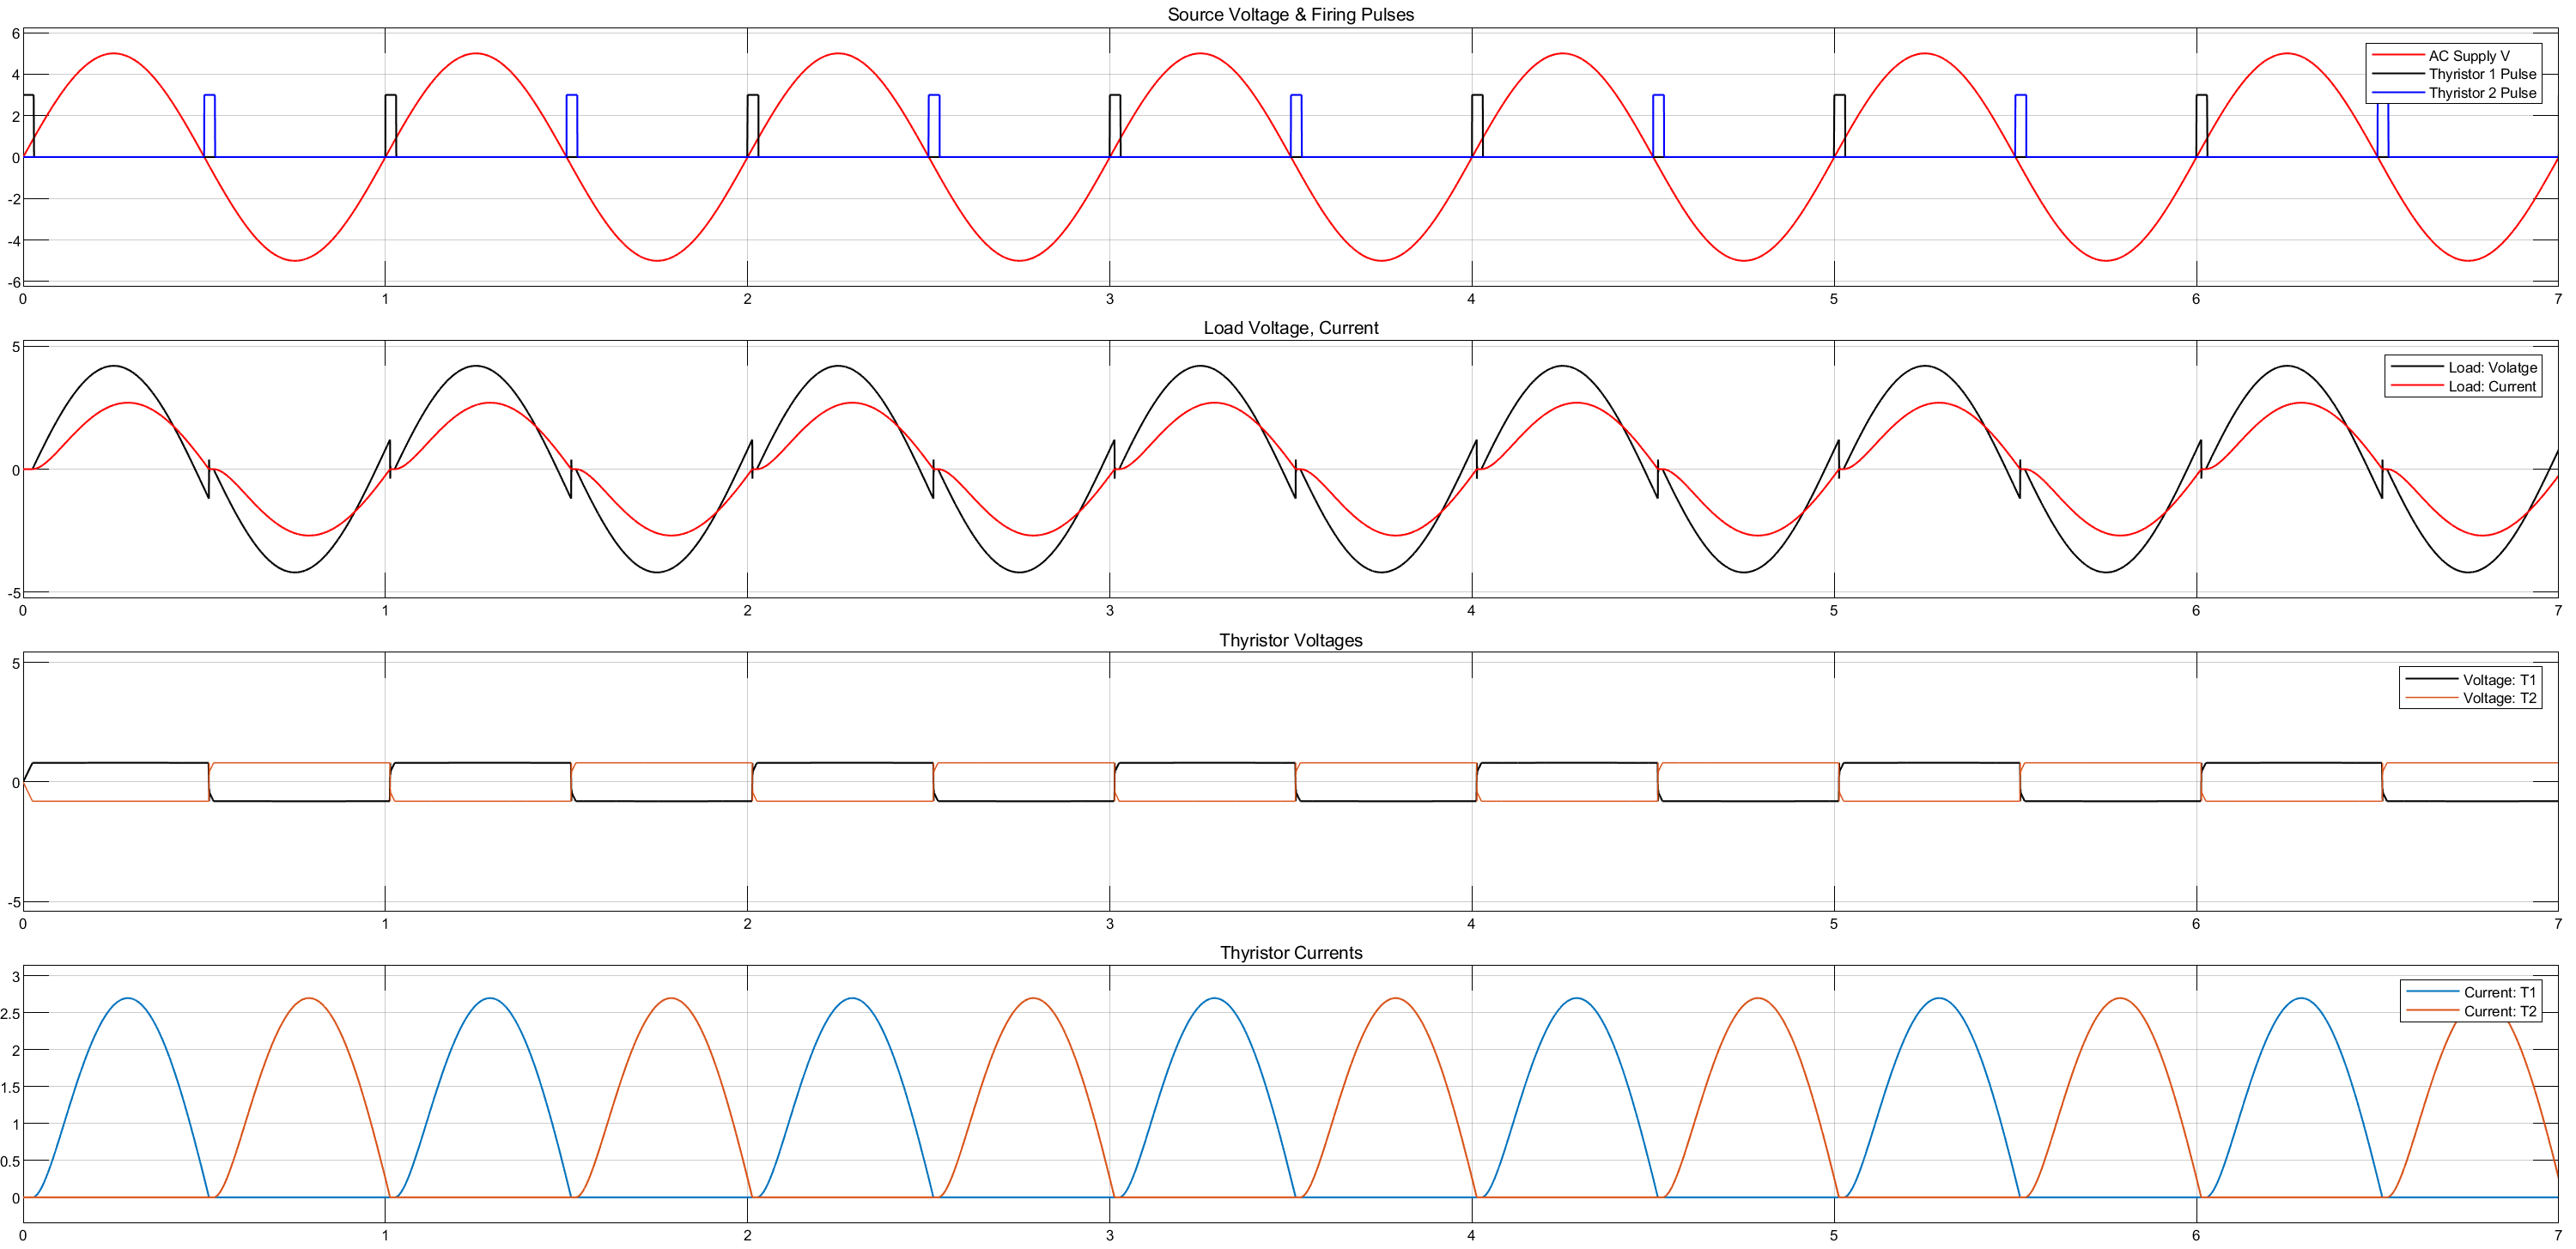
\includegraphics[width=\textwidth]{2RLnd.png}
    \caption{Simulation Output for RL Load, Controlled Rectifier, No Delay}
    \label{fig:rControlledWithDelay}
\end{figure}

\begin{figure}[H]
    \centering
    % 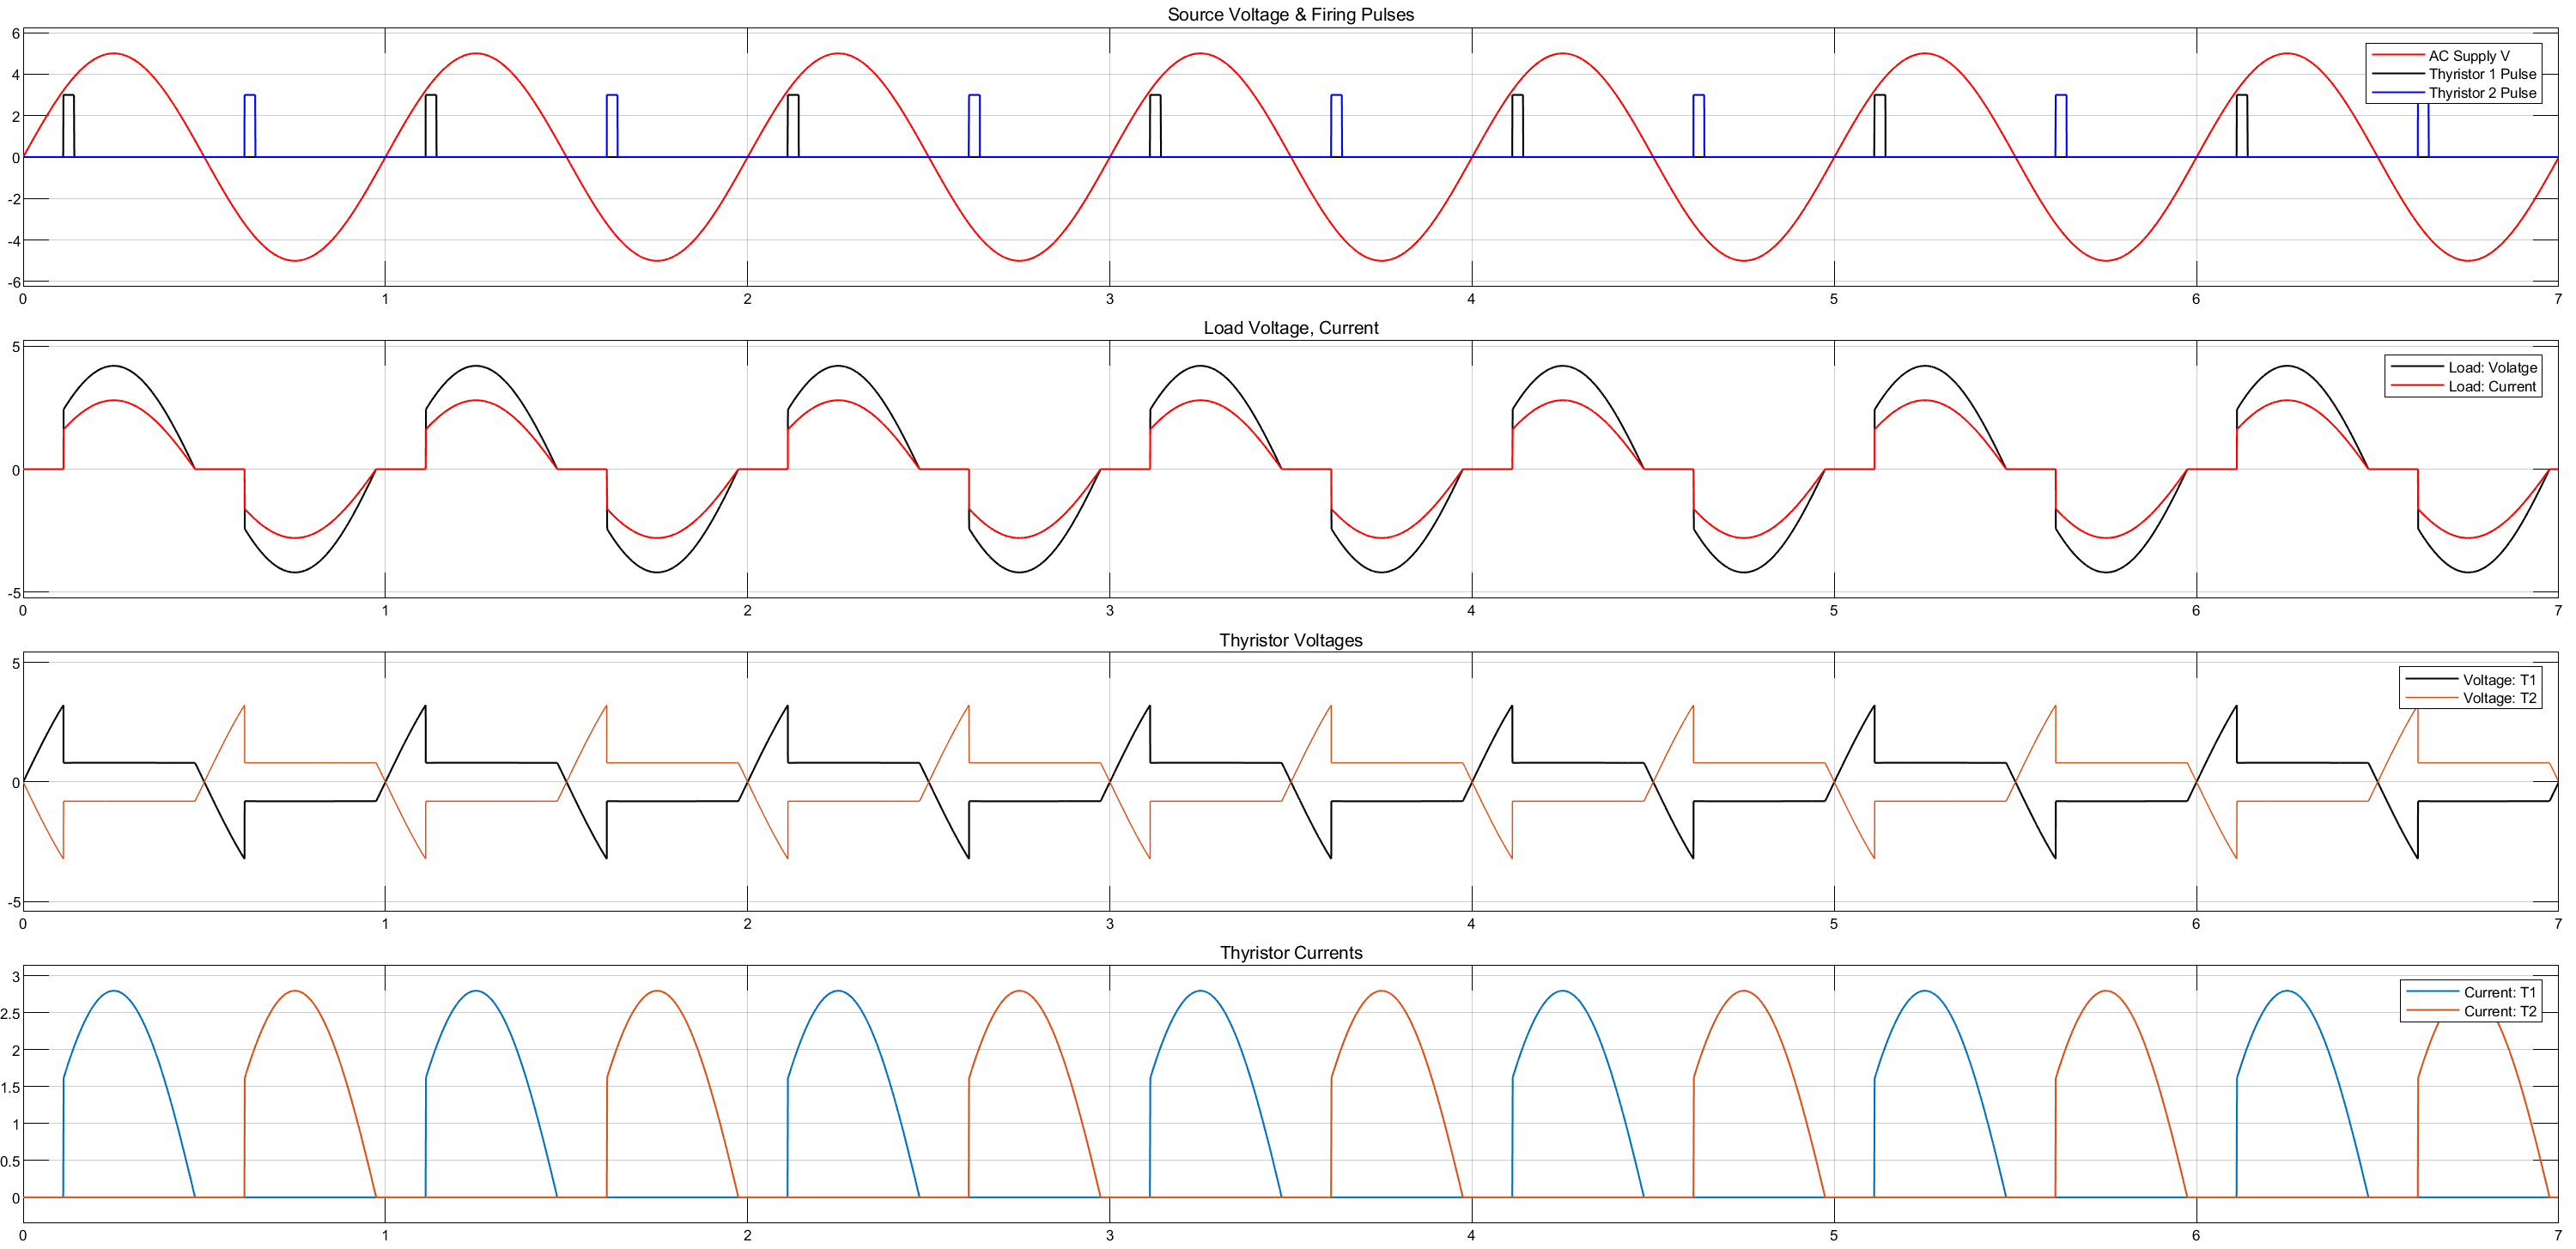
\includegraphics[width=\textwidth]{3Rd.png}
    \caption{Simulation Output for R Load, AC-AC Bidirectional Voltage Controller}
    \label{fig:rLoad}
\end{figure}

\begin{figure}[H]
    \centering
    % 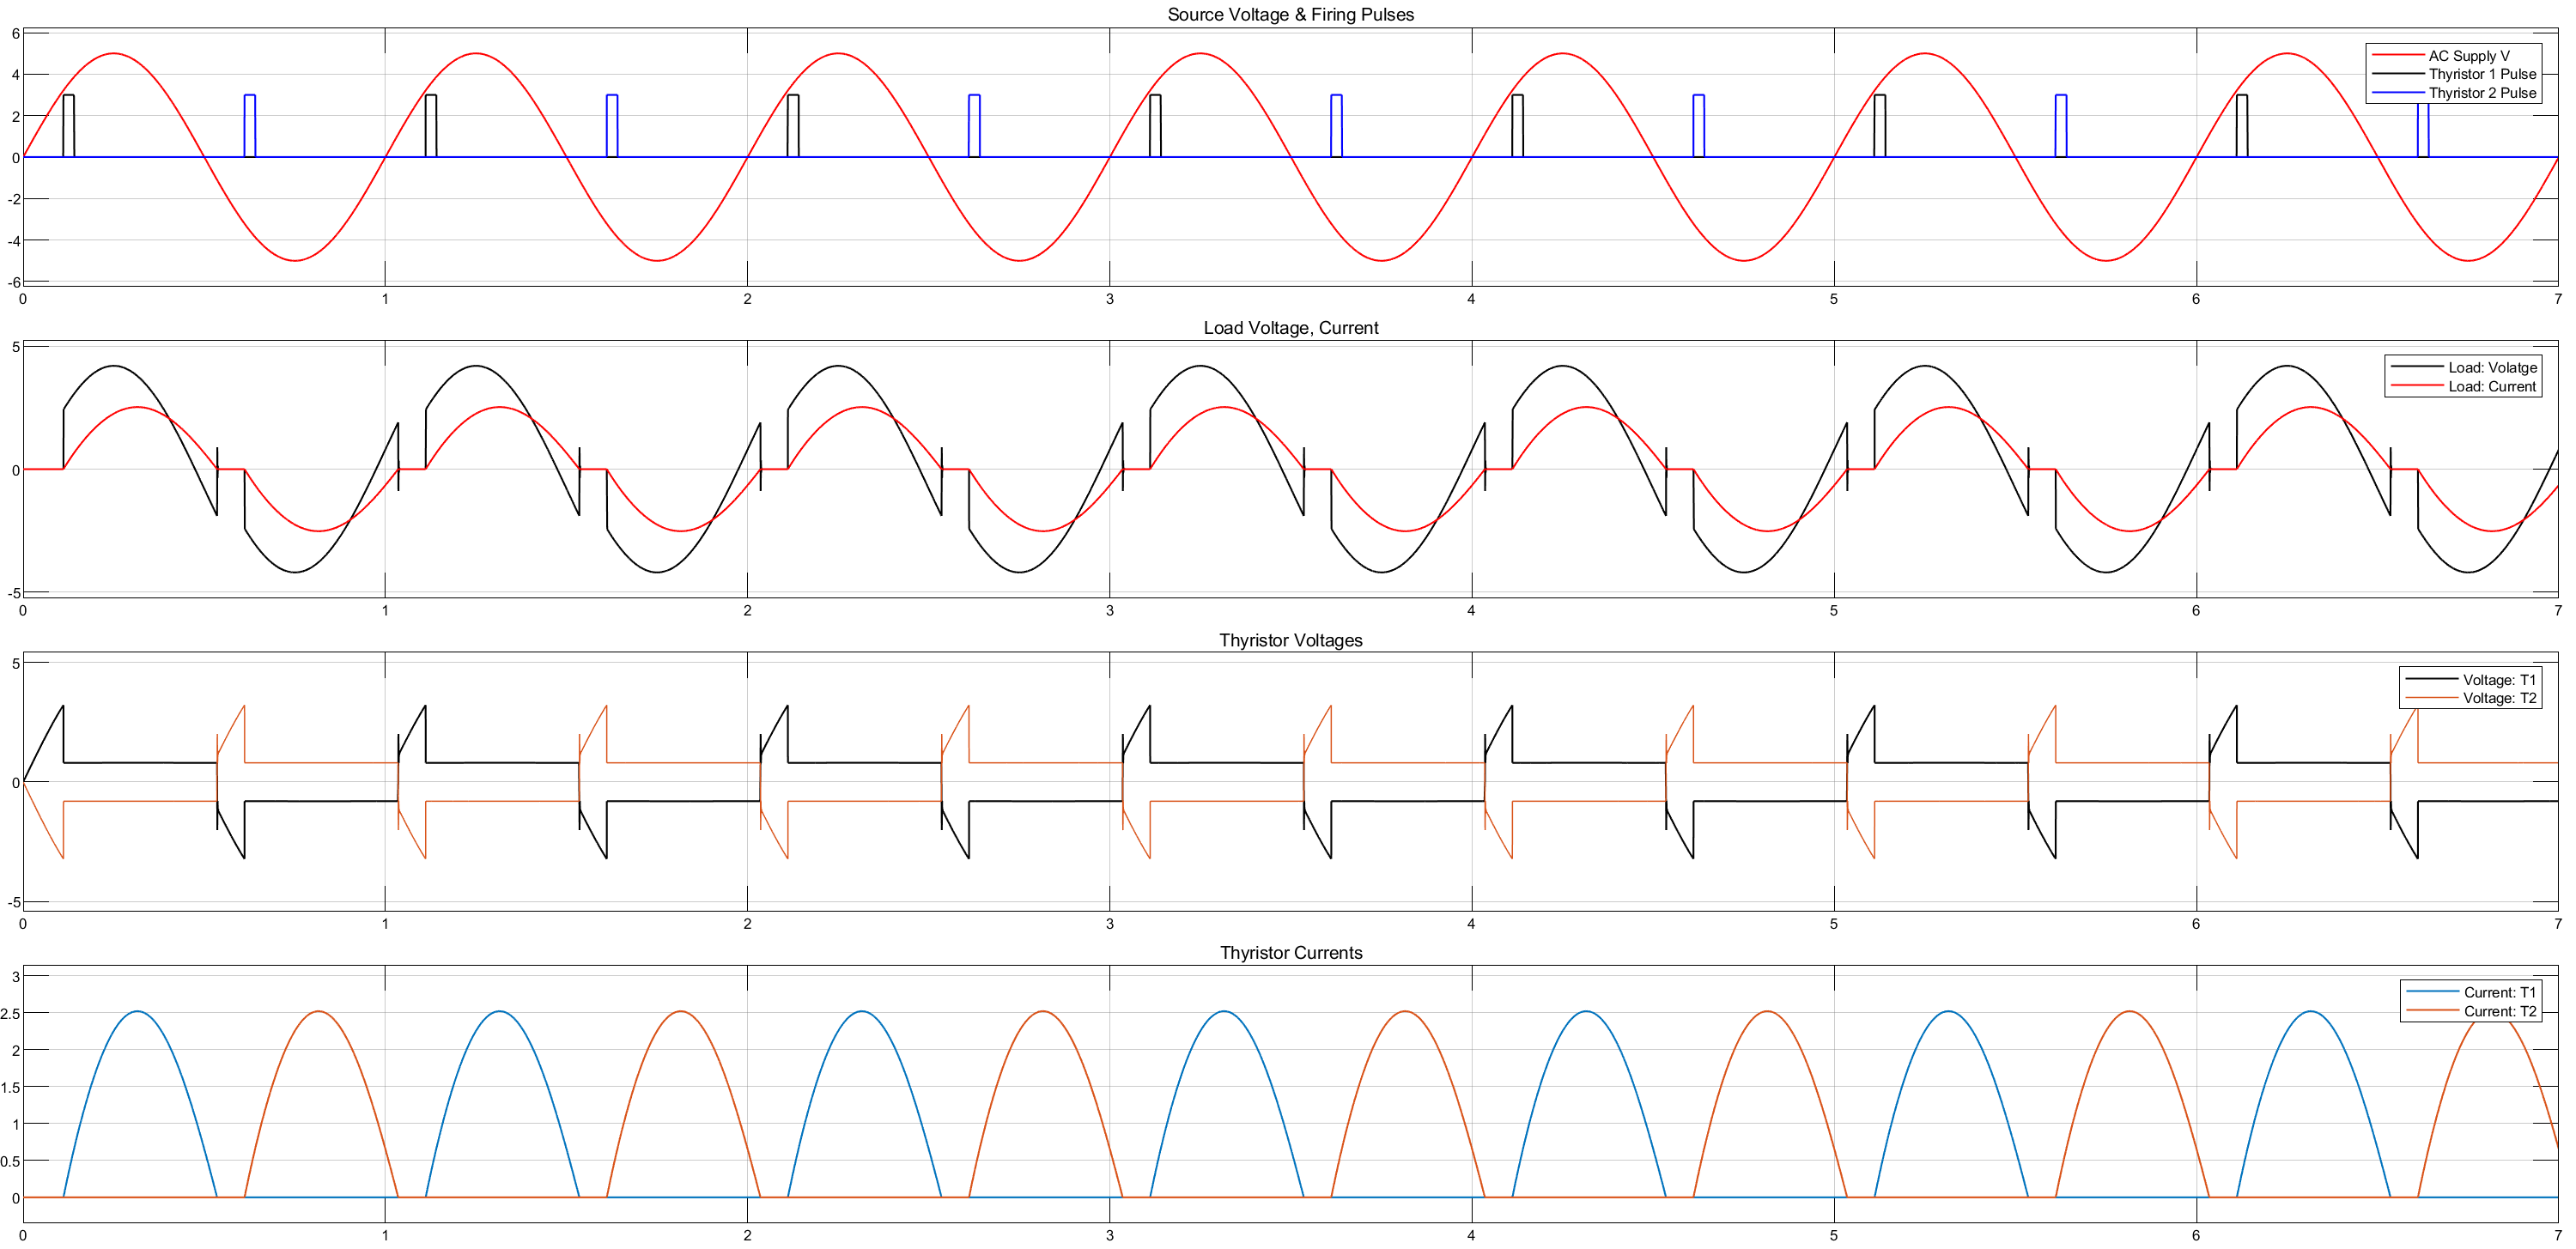
\includegraphics[width=\textwidth]{4RLd.png}
    \caption{Simulation Output for RL Load, AC-AC Bidirectional Voltage Controller}
    \label{fig:rlLoad}
\end{figure}


\section*{Discussion}
\addcontentsline{toc}{section}{Discussion}
The Single Phase Bridge Inverter is a crucial circuit for converting DC power to AC power, enabling the operation of AC loads from a DC source. Through MATLAB/Simulink simulations, we analyzed the behavior of the inverter under resistive (R) and inductive (RL) loads. The results demonstrate the impact of switching patterns on the output voltage and current waveforms. For R loads, the current waveform closely follows the voltage waveform, while for RL loads, the current lags the voltage due to inductance, affecting the conduction period of the freewheeling diodes.

\section*{Conclusion}
\addcontentsline{toc}{section}{Conclusion}
The study of the Single Phase Bridge Inverter with R and RL loads highlights its effectiveness in converting DC to AC power and controlling the output waveform through switching patterns. The circuit's behavior under different load conditions underscores the importance of considering load characteristics in inverter design and operation. MATLAB/Simulink simulations provide valuable insights into the inverter's performance, enabling optimization for industrial applications such as motor drives, renewable energy systems, and uninterruptible power supplies.

\bibliographystyle{IEEEtran}
\renewcommand{\bibname}{References}
\addcontentsline{toc}{section}{References}
\bibliography{ref}

\end{document}
